\documentclass[12pt]{scrartcl}

\usepackage{fontspec}
\usepackage{polyglossia}
\setdefaultlanguage{russian}
\newcommand{\docfont}{Times New Roman}
\setmainfont[Ligatures=TeX]{\docfont}
\newfontfamily\cyrillicfont[Ligatures=TeX]{\docfont}
\newfontfamily\cyrillicfontsf[Ligatures=TeX]{\docfont}
\newfontfamily\cyrillicfonttt[Ligatures=TeX]{\docfont}

\usepackage{amsmath,amsfonts,amsthm} % nice math symbols
\newtheorem{definition}{Определение}
\usepackage{hyperref}
\hypersetup{%
	pdfencoding=auto,
	pdfauthor={Александр Панов},
	pdftitle={Операции в знаковой картине мира}
}
\usepackage{csquotes}
\usepackage{graphicx}
\graphicspath{{../../images/}}

\usepackage[
%	autolang=hyphen,
	language=auto,
	autolang=other,
	backend=biber,
	style=gost-numeric
]{biblatex}
\addbibresource{../../biblio/library.bib}
\DeclareSourcemap{
	\maps[datatype=bibtex, overwrite]{
		\map{
			\step[fieldset=langid, fieldvalue=english]
			\step[fieldset=doi, null]
			\step[fieldset=issn, null]
			\step[fieldset=isbn, null]
			\step[fieldset=url, null]
			\step[fieldsource=language, fieldset=langid, origfieldval]
		}
	}
}

\linespread{1.3}

\title{Операции в знаковой картине мира}
\author{Осипов~Г.\,С., Панов~А.\,И.\\
	{\large\slshape ФИЦ ИУ РАН, пр. 60-летия Октября, 9, gos@isa.ru}}

\begin{document}
%	\affil{ФИЦ ИУ РАН}
	
	\maketitle{}
	\begin{abstract}
		В работе рассмотрен
		\par\bigskip
		\textit{Ключевые слова}: знаковая картина мира, образ, значение, личностный смысл.
	\end{abstract}
	
	
	
	\section*{Введение}
	Про постановку задачи \cite{Osipov2014c,Osipov2015d}.
	
	Психологические и нейрофизиологические основания трехкомпонентной структуры знака.
	
	\section{Картина мира}

	Про компоненты знака, функции связывания и три типа картин мира.
	
	Введем два знака,~которые мы будем рассматривать на протяжении всей статьи в качестве примеров, иллюстрирующих положения, которые приводятся в настоящей работе.
	
	
	\section{Строение компонент знака}
	
	До именования знак будем называть протознаком или признаком.
	Будем считать, что входной поток данных представляет собой последовательность векторов или событий. События представляют собой бинарные векторы 
	
	\begin{figure}[h]
		\centering
		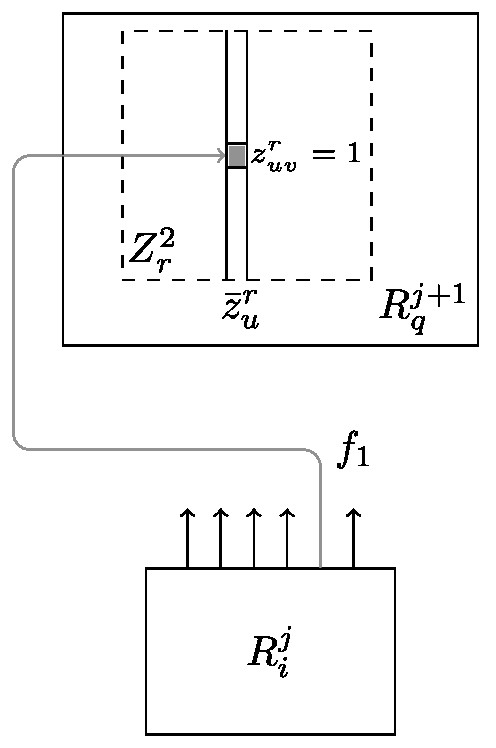
\includegraphics[width=0.3\linewidth]{automata/meas}
		\caption{Определение отношения включения на множестве признаков.}
		\label{fig:rb_measure}
	\end{figure}
	
	Все признаки, которые включаются в признак $f$ формируют входное множество $F_{in}$ признака $f$: $F_{in}(f)=\{f_i|f_i\sqsubset f\}$. Соответственно, все признаки, которые включают в себя признак $f$ формируют выходное множество $F_{out}$ признака $f$: $F_{out}(f)=\{f_i|f\sqsubset f_i\}$. Будем называть два признака $f_1$ и $f_2$ равными по входным множествам, или $f_1 \asymp f_2$, если $F(f_1)=F(f_2)$. Иными словами, по входными множествам формируются классы эквивалентности признаков. Такие классы эквивалентности будем называть узлами.
	
	Введем специальную процедуру $\Lambda$, которая позволяет разделить множество столбцов матриц предсказания для каждого признака $f$ на два подмножества: $\Lambda(Z(f))=(I^c,I^e)$, где $I^c=\{i_1^c,i_2^c,\dots\}$ --- индексы столбцов-условий, $I^e=\{i_1^e,i_2^e,\dots\}$ --- индексы столбцов-эффектов . Действие процедуры $\Lambda$ заключается в поиске причинно-следственных связей во входном множестве признака $f$ или, иными словами, в установлении частичного порядка на множестве столбцов матриц предсказания. 
	
	Справедливы следующие утверждения относительно свойств процедуры $\Lambda$:
	\begin{itemize}
		\item $I^c\cap I^e=\emptyset$ --- столбец матрицы предсказания не может быть одновременно и условием и эффектом,
		\item $|I^c\cup I^e|=h$ --- столбец матрицы предсказания является либо условием либо эффектом,
		\item $I^c\not = \emptyset$ --- среди столбцов матрицы предсказания должен быть хотя бы один столбец условий, в то время как эффектов может и не быть (в случае объектных признаков),
		\item $\forall i\in I^e, j\in I^c\ i>j$ --- все условия предшествуют эффектам по времени.
	\end{itemize}
	
	Перцептом признака мы будем называть входное множество, а значением --- выходное.
	
	\section{Отношения в семиотической сети}
	\subsection{Семиотическая сеть}
	Пусть $W=\langle \boldsymbol Z,\boldsymbol F,H,R_Z\rangle$, где $\boldsymbol Z$ --- множество всех матриц предсказания, $\boldsymbol F$ --- множество всех признаков, $H=\{\sqsubset^1, \sqsubset^2, \dots\}$ --- семейство базовых отношений на множестве $\boldsymbol F$: отношения включения признаков по столбцу $t_1,t_2,\dots$, $R_Z$ --- семейство отношений на множестве признаков, формируемых на основе структуры матриц $\boldsymbol Z$. Каждому признаку $f$ соответствует набор матриц предсказания $Z(f)\subseteq \boldsymbol Z$, а каждой матрице предсказания $Z_i\in Z(f)$ --- набор входных признаков $F(Z_i)=F_{in}(f)$. 
	
	Далее мы будем описывать возможные отношения семейства $R_Z$. Рассмотрим два признака $f_1$ и $f_2$. На первом этапе будем считать, что $Z(f_1)=\{Z_1\}, Z(f_2)=\{Z_2\}$, т.е. каждый признак определяется только одной матрицей предсказания. Затем обобщим определенный нами отношения на общий случай с несколькими матрицами предсказания.

	\subsection{Отношения на множестве образов}	
	\begin{definition}[Отношение эквивалентности]
		Если 
	\end{definition}
	
	
	Отношение включения по событиям и включения по признакам.
	
	Отношение противопоставления и сходства.
	

	\section{Операции в семиотической сети}
	Отношения на сети реализуются с помощью соотношений матриц предсказания. Операции осуществляется в одной сети --- как это сказывается на компонентах знака в другой сети, как они преобразуются. Содержательной описание операций. Пример: обобщение на сети образов для знаков <<яблоко>> и <<апельсин>> общее значение не включает в себя действие <<чистить>>, т.к. не присутствуют все необходимые признаки в обобщенном образе (нет ссылки на знак <<кожура>>).
	
	\subsection{Операции обобщения}
	
	\subsection{Операция актуализации}
	
	\subsection{Операции логического вывода}
	
	\section*{Заключение}
	
	\printbibliography
\end{document}